\section{Data Sources}\label{sec:data}

We use the TLC Yellow Taxi Trip Records~\cite{tlc_data} for January 2023 to December
2024. Each month is published as an Apache Parquet file with one row per trip and
about twenty columns, together with a lookup table that maps the 265 taxi-zone IDs to
zone and borough names. \texttt{scripts/prepare\_data.py} downloads the files and
converts each month to a header-less CSV with the eight columns the jobs need;
\cref{tab:schema} shows them with the first trip of January 2024. CSV is used because
Hadoop Streaming feeds mappers with lines of text.

\begin{table}[t]
\centering
\caption{Columns used, with the first trip of January 2024 as an example}\label{tab:schema}
\setlength{\tabcolsep}{4pt}
\begin{tabularx}{\columnwidth}{@{}>{\ttfamily}ll>{\raggedright\arraybackslash}X@{}}
\toprule
\normalfont Column (TLC name) & Example & Use \\
\midrule
tpep\_pickup\_datetime & 2024-01-01 00:57:55 & hour (\texttt{demand}) \\
PULocationID & 186 (Penn Station) & pickup zone \\
DOLocationID & 79 (East Village) & drop-off zone \\
trip\_distance & 1.72 (miles) & band; cleaning \\
fare\_amount & 17.70 (US\$) & mean fare \\
tip\_amount & 0.00 (US\$) & tip rate \\
total\_amount & 22.70 (US\$) & not used \\
payment\_type & 2 (cash) & 1 = card: tip known \\
\bottomrule
\end{tabularx}
\end{table}

\begin{figure*}[t]
\centering
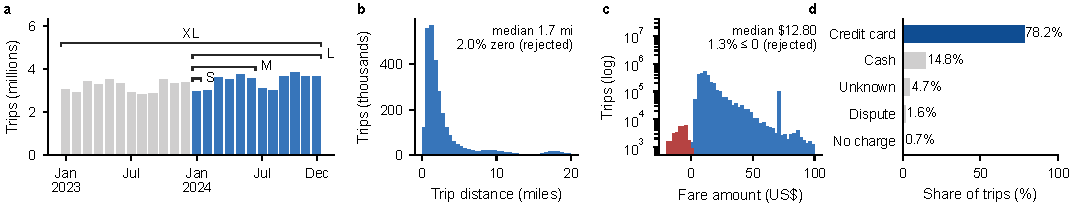
\includegraphics[width=\textwidth]{figures/data_overview.pdf}
\caption{What the input looks like. (a)~Yellow-taxi trips per month, January 2023 to
December 2024 (Parquet row counts), and the nested tiers S, M, L and XL.
(b)--(d)~January 2024: (b)~trip distance up to 20~miles, (c)~fare amount (log scale;
red: zero or negative fares, which are rejected), (d)~payment types.}\label{fig:data}
\end{figure*}

\Cref{fig:data} shows what the records look like. Demand is steady at 2.8--3.8~million
trips per month (lowest in August 2023, highest in October 2024), so every month adds a
similar amount of work. Most trips are short: the median distance is 1.7~miles and the
median fare US\$12.80. The spike at US\$70 is the flat fare between JFK Airport and
Manhattan (3.3\% of the trips). 78\% of the trips are paid by credit card, the only
payment type for which tips are recorded; 15\% are paid in cash.

To study how scaling depends on data size, the months are grouped into nested tiers
(\cref{tab:tiers}). Every monthly file is 140--180\,MiB, i.e.\ two 128\,MB HDFS
blocks, so Hadoop starts about two map tasks per month: 2 for tier S but 48 for
tier XL. Tiers S, M, L and XL are used for strong scaling; W3 and W9 complete the
weak-scaling series of three months per worker (W3, M, W9, L for 1--4 workers).

\begin{table}[t]
\centering
\caption{Dataset tiers (valid = rows passing the cleaning rules)}\label{tab:tiers}
\begin{tabular*}{\columnwidth}{@{\extracolsep{\fill}}llrrr@{}}
\toprule
Tier & Period & Rows & Valid & CSV size \\
\midrule
S  & Jan 2024 (1 mo.)       & \num{2964624}  & 96.8\% & 142\,MiB \\
W3 & Jan--Mar 2024 (3 mo.)  & \num{9554778}  & 96.4\% & 457\,MiB \\
M  & Jan--Jun 2024 (6 mo.)  & \num{20332093} & 96.7\% & 974\,MiB \\
W9 & Jan--Sep 2024 (9 mo.)  & \num{30021209} & 96.6\% & 1.40\,GiB \\
L  & 2024 (12 mo.)          & \num{41169720} & 96.4\% & 1.93\,GiB \\
XL & 2023--2024 (24 mo.)    & \num{79479946} & 96.7\% & 3.72\,GiB \\
\bottomrule
\end{tabular*}
\end{table}

\textbf{Data quality.} The raw records contain zero or negative distances and fares
(2.0\% and 1.3\% of the trips in January 2024), implausible values and missing payment
types. Records failing the rules in \cref{sec:algorithm} are dropped: \num{1464575} of
\num{41169720} rows (3.6\%) in tier L and \num{2587058} (3.3\%) in tier XL. Tips are
analysed only for credit-card trips, because cash tips are not recorded.
